\chapter{Úvod}
\blindtext

Cílem této bakalářské práce je vytvořit webovou aplikaci typu kanban určenou pro řízení projektů na základě požadavků společnosti SEACOMP s.r.o. Za tímto účelem je společností v současné době využíván nástroj třetí strany, který ovšem není plně přizpůsoben potřebám této společnosti, ku příkladu není integrován do dalších interních aplikací.

Téma práce mne zaujalo zejména díky stále rostoucí popularitě interaktivních webových aplikací, motivující pro mne bylo mít možnost takovou aplikaci implementovat naprosto sám. Také mne lákala možnost firemního zadání bakalářské práce, díky kterému bude mít výsledná reálné využití a bude využívána v praxi. 

\blindtext

\chapter{Rozbor řešené problematiky}
V úvodu této kapitoly jsou stručně shrnuty populární metodiky řízení projektů s větším zaměřením na metodiky agilní a to především na metodiku Kanban. V další části kapitoly je představeno několik již existujících aplikací umožňujících využívat právě tuto zmíněnou metodiku. Dále je text věnován zmapování infrastruktury zadavatele této práce a jeho požadavkům na výslednou aplikaci. Závěr kapitoly obsahuje popis technologií, které byly využity pro tvorbu této bakalářské práce.

\section{Metodiky řízení projektů}
Obecně lze metodiky používané pro řízení softwarových projektů rozdělit do dvou hlavních kategorií. Jedná se o tradiční metodiky a metodiky agilní.

Jak název napovídá, tradiční metodiky mají delší historii. Lidstvo potřebovalo využívat řízení projektů již odpradávna, exemplárním příkladem jsou obrovské stavební projekty jako pyramidy v Gíze nebo Velká čínská zeď. Tyto projekty jistě vyžadovaly důkladné řízení jak pracovních sil, tak i přísunu materiálu a dalších. Výsledek musel bezpochyby také splňovat určité požadavky. Ohledně metodik takovýchto plánování ovšem neexistuje příliš mnoho dokumentace. K určité standardizaci řízení projektů totiž začalo docházet až v padesátých letech minulého století. Značný podíl zde má i Námořnictvo Spojených států amerických a to konkrétně Projekt Manhattan\footnote{Krycí název pro projekt vývoje atomové bomby během druhé světové války}~\cite{bib:project-managment-history}.

Rozdílem mezi dvěma zmíněnými kategoriemi řízení projektů je především strukturace procesů. U tradičních metod probíhají tyto procesy sekvenčně, tento přístup zpravidla vyžaduje důkladnější počáteční plánování a pozdější změny požadavků mnohdy představují náročný problém. Oproti tomu při použití agilních metod jsou jednotlivé procesy úzce spjaty a pracuje se v iteracích. Díky tomu je do vývoje více zapojen zákazník a takovýto projekt se snadněji vypořádá s případnými změnami požadavků~\cite{bib:agile-vs-traditional}. 

Populárním zástupcem tradičních metodik je například vodopádový model (znázorněný diagramem~\ref{img:waterfall}), na kterém je na první pohled patrné právě sekvenční řazení jednotlivých procesů vývoje. Tento model se objevil koncem šedesátých let minulého století, kdy byly programovací jazyky neefektivní, procesory pomalé a paměť počítačů byla výrazně omezená~\cite{bib:agile-history}. 

\begin{figure}[H]
	\centering
	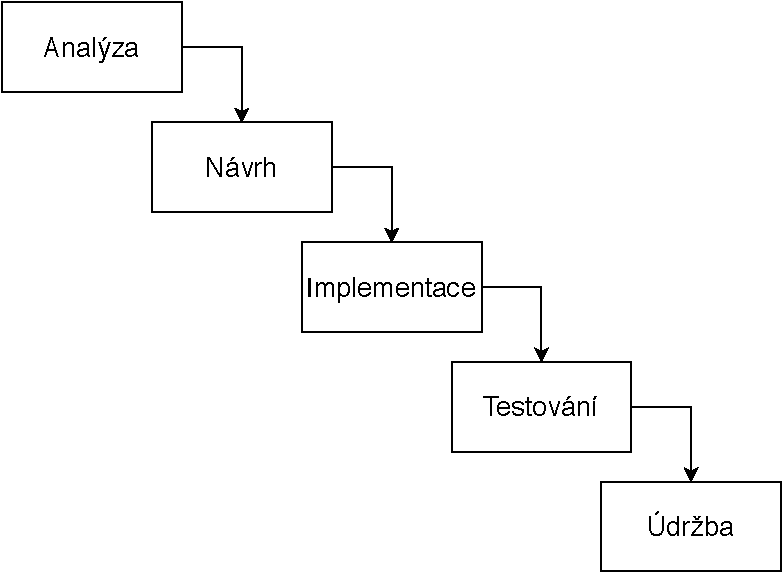
\includegraphics[width=\textwidth]{obrazky-figures/waterfall.pdf}
	\caption{Grafické znázornění posloupnosti jednotlivých procesů tradiční metodiky řízení projektů označované jako vodopádový model.}
	\label{img:waterfall}
\end{figure}

U tradičních metodik je předpokladem, že se k dokončeným fázím projektu již nebude nutné vracet. Takový předpoklad lze aplikovat na mnoho odvětví. Příkladem budiž stavba budovy, u které je nutné nejprve řádně celý projekt naplánovat a zdokumentovat. Jakmile samotná stavba započne, větší změny oproti původnímu projektu vznikají velmi zřídka. V oblasti informačních technologií, obzvláště při vývoji softwaru, však odchýlení od původního plánu nebývá žádnou výjimkou. Řízení projektů tohoto typu pomocí striktních tradičních metodik je tedy často obtížné a značně neefektivní~\cite{bib:agile-vs-traditional-what}.

V dnešní době se stává častěji než tomu bylo v minulosti, že se softwarové projekty během vývoje mění, narůstají jejich požadavky, přibývají funkce a to vše i během jejich vývoje. Tento trend se týká především webových systémů. Jako reakce na tyto náhlé změny byly v devadesátých letech stvořeny právě agilní metodiky~\cite{bib:agile-history}. 

\subsection{Agilní metodiky řízení projektů}
Agilní metodiky jsou skupina metod řízení projektů určena především pro vývoj softwaru. 

Veřejný zájem o tyto metodiky začal až v pozdních devadesátých letech~\cite{bib:agile-mobile}. V roce 2001 se v Utahu sešlo sedmnáct zastánců agilních metodik a sestavilo Manifest Agilního vývoje software, který vystihuje čtyři hlavní zásady těchto metod~\cite{bib:agile-manifest}.
\begin{itemize}
  \item Jednotlivci a interakce před procesy a nástroji
  \item Fungující software před vyčerpávající dokumentací
  \item Spolupráce se zákazníkem před vyjednáváním o smlouvě
  \item Reagování na změny před dodržováním plánu
\end{itemize}

Tyto metodiky jsou více zaměřené na lidi a na jejich vzájemnou komunikaci. To je jedním z důvodů, proč jsou agilní metodiky vhodné především pro menší týmy. Díky absenci sekvenčního řazení procesů vývoje tyto metody také zvyšují efektivitu nepředvídatelných a stále se měnících projektů. Vypuštěním striktního plánování je také možné projekt dokončit rychleji než použitím tradičních metodik.

Vývoj řízený agilními metodikami (znázorněný diagramem~\ref{img:agile}) probíhá iterativně a inkrementálně. Na začátku vývoje se určí základní požadavky a postupnými cykly se tyto požadavky zdokonalují. Jedna iterace takového vývoje trvá zpravidla jeden týden až měsíc. Během této iterace proběhne celý cyklus vývojových procesů (podobně jako u vodopádového modelu znázorněného diagramem~\ref{img:waterfall}). Dokončením iterace vzniká prototyp, který může být prezentován zákazníkovi. Díky tomu získává přesnější představu o podobě produktu a lze včas odhalit nedostatky požadavků, které dříve nebyly známy~\cite{bib:agile-impact}.

\begin{figure}[H]
	\centering
	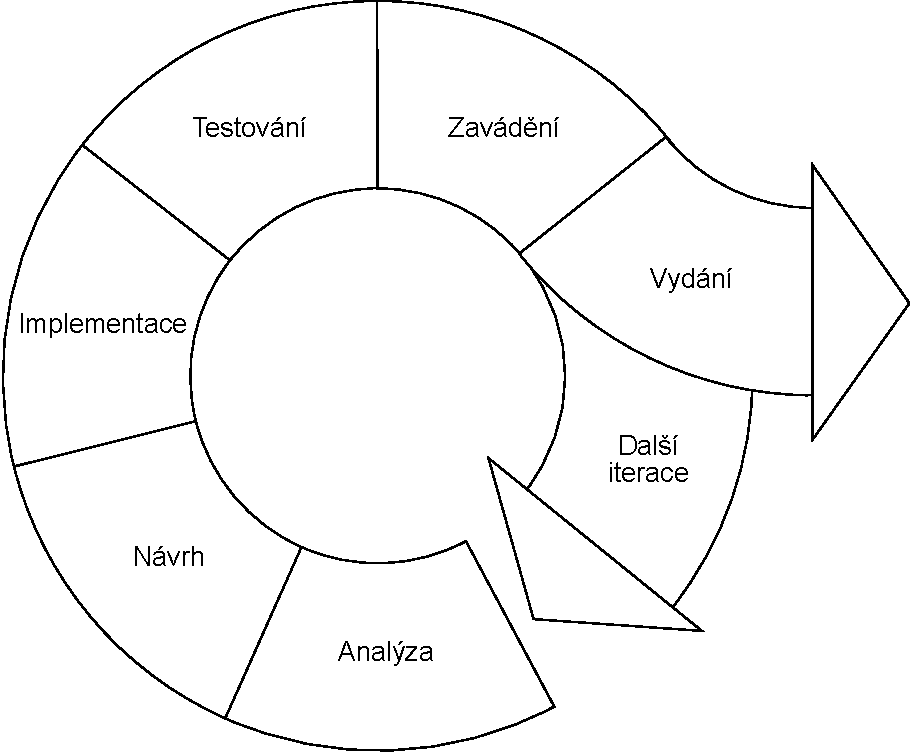
\includegraphics[width=\textwidth]{obrazky-figures/agile.pdf}
	\caption{Grafické znázornění posloupnosti jednotlivých procesů agilních metodik řízení projektů.}
	\label{img:agile}
\end{figure}

Mezi populární agilní metodiky patří například Scrum, Lean Developmet, Extrémní programování (angl. \emph{Extreme Programming} nebo také XP), Crystal, Vlastnostmi řízený vývoj (angl. \emph{Feature Driven Development} neboli FDD) a v neposlední řadě také Kanban.

\blindtext % vyzaduje spolupraci

Jedna ze studií na toto téma uvádí, že ze 1386 sledovaných projektů 65\% z nich využilo během vývoje agilní metody a 6\% projektů bylo dokončeno téměř pouze s použití agilních metod~\cite{bib:agile-work}. % @todo dopsat cisla uspechu

\subsection{Metodika Kanban}
Kanban je slovo převzaté z japonského jazyka, kde znamená \uv{cedule}. Toto slovo je taktéž spjato s poslední výzvou k objednávce před uzavřením podniku (sundáním cedule). Takovou objednávku lze označit jako \uv{na poslední chvíli} nebo také jako objednávku \uv{tak akorát na čas}~\cite{bib:dict-kanban}. 

Tak akorát na čas (anglicky \emph{Just-in-time}) je filozofie řízení výroby, vyvinuta v sedmdesátých létech japonskou automobilovou společností Toyota Motor Corporation\footnote{Toyota Motor Corporation: \url{https://global.toyota/en/}}. Hlavní myšlenkou toho přístupu je mít přesné množství materiálu, na správném místě a ve správný čas. Díky tomu dochází k redukci množství materiálu, který aktuálně není zpracováván a nemělo by docházet k jeho přebytečnému hromadění~\cite{bib:just-in-time}.

\begin{figure}[H]
	\centering
	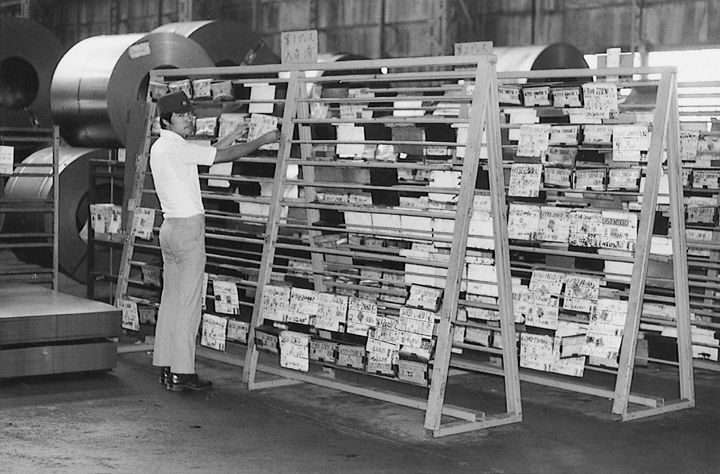
\includegraphics[width=\textwidth]{obrazky-figures/toyota-kanban.jpg}
	\caption{Původní provedení kanbanu v továrně společnosti Toyota Motor Corporation \emph{Převzato z~\cite{bib:toyota-history}}.}
\end{figure}

\blindtext[2] %todo Popsat princip (přesouvání apod), možná ukázka sticky note?

\section{Aplikace s podobným zaměřením}
Jelikož je metodika Kanban existuje již několik několik desítek let, lze v dnešní době nalézt celou řada programů a webových aplikací, které je možné pro aplikování této metodiky využít. V této podkapitole je několik takových aplikací stručně přiblíženo a jsou vyzdviženy některé jejich klíčové vlastnosti. Pro bližší představu o podobě těchto aplikací je každá z nich doprovázena snímkem obrazovky. Jedná se o dva populární zástupce z řad produktů společnosti Atlassian -- aplikace Trello a Jira. Třetí představenou aplikací je o něco méně známá aplikace Kanboard, která je však v současné době využívaná společností SeaComp.

\subsection{Trello}
Trello\footnote{Trello: \url{https://trello.com}} je především webová aplikace provozovaná v současné době společností Atlassian\footnote{Atlassian: \url{https://www.atlassian.com}}. Historie této aplikace sahá až do roku 2011, kdy byla veřejně spuštěna jako webová aplikace a také jako aplikace pro platformu iOS. K dnešnímu dni je aplikaci Trello možné navíc využít i na mobilní platformě Android nebo jako program pro operační systémy Microsoft Windows či macOS. 

Během několika let své existence se aplikace stala velice populární a našla si několik milionů uživatelů. K věhlasným společnostem, které tuto aplikaci využívají patří například technologický gigant Google\footnote{Google: \url{https://about.google/}}, softwarová společnost Red Hat\footnote{RedHat: \url{https://www.redhat.com/en/about/company}} nebo platforma pro skupinové financování Kickstarter\footnote{Atlassian: \url{https://www.kickstarter.com/about}}~\cite{bib:trello-about}. 

Svou velkou popularitu si aplikace zasloužila především přívětivým uživatelským rozhraním a jednoduchostí použití. Cesta od první návštěvy stránky k práci na své první Kanban nástěnce uživatele dělí doslova minuty. Pro základní použití navíc bez problému vystačí bezplatná verze aplikace. Díky těmto faktům Trello není využíváno pouze softwarovými společnostmi, ale lze ho použít například i jako osobní seznam úkolů~\cite{bib:jira-vs-trello}.

Trello nabízí řadu vylepšení, díky kterým je možné nástěnku rozšířit o funkce z aplikací třetích stran. 
% https://help.trello.com/article/1094-what-are-power-ups
V bezplatné verzi lze však využít pouze jedno vylepšení.
% https://trello.com/cs/pricing
Nástěnka je umístěna na vzdáleném úložišti a službu nelze provozovat na svém vlastním serveru. Nicméně mobilní aplikace umožňují pracovat s nástěnkami i bez přístupu k internetu.
% https://blog.trello.com/trello-common-questions

\begin{figure}[H]
	\centering
	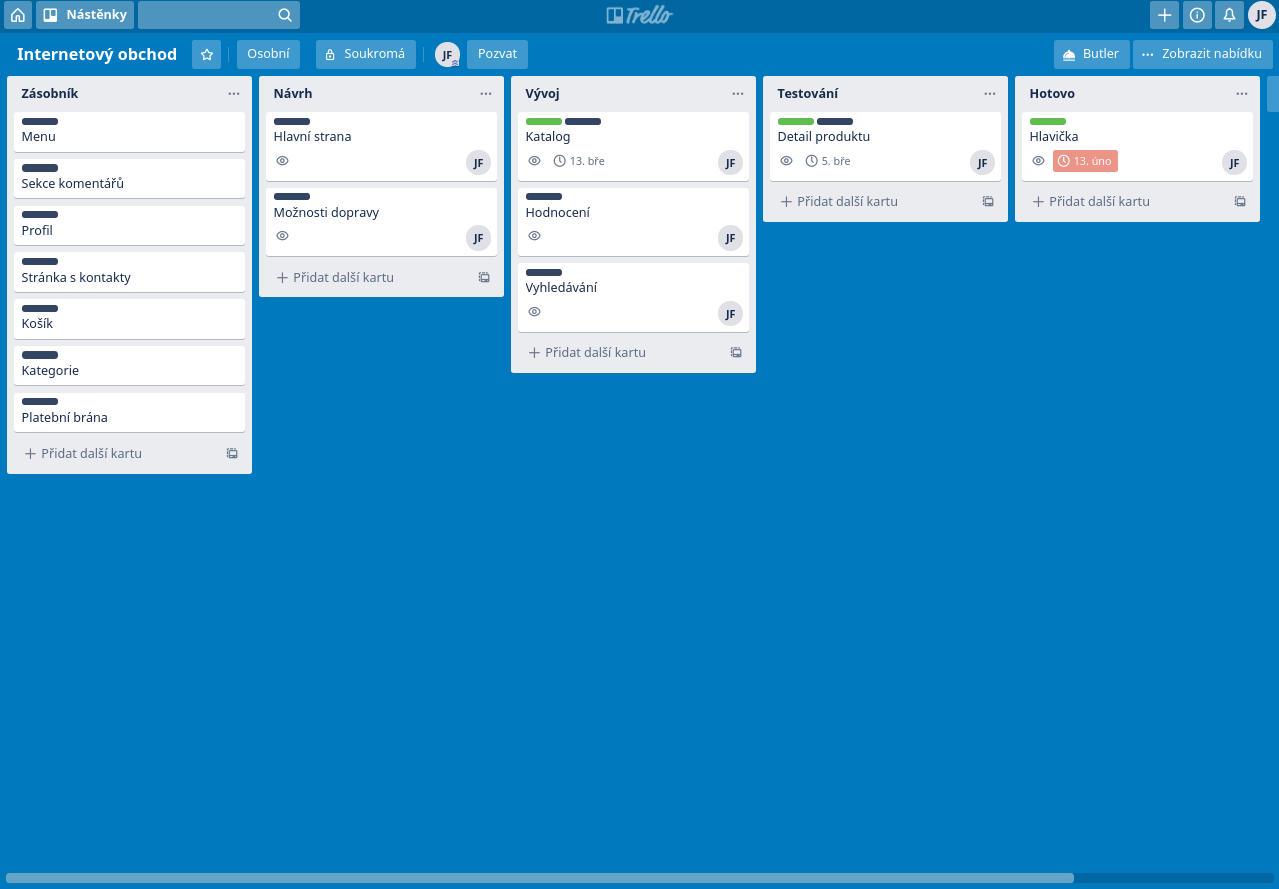
\includegraphics[width=\textwidth]{obrazky-figures/trello.png}
	\caption{Vzorová Kanban nástěnka ve webové aplikaci Trello zaměřená na vývoj internetového obchodu.}
\end{figure}

\subsection{Jira}
Jira\footnote{Jira: \url{https://www.atlassian.com/cs/software/jira}} je řada produktů společnosti Atlassian, určená ke správě práce v nejrůznějších typech týmů. Nástěnka Kanban je součást například produktu Jira Software, který je určen pro vývojáře softwaru. 
% https://www.atlassian.com/software/jira/guides/getting-started/overview#jira-software-hosting-options

% Co má navíc oproti Trellu, pluginy

% @todo platformy

Tato aplikace je využívána více něž 65 tisíci zákazníky po celém světě mezí které se řadí například internetovou aukční síň eBay\footnote{eBay: \url{https://www.ebayinc.com/company/}}, služba pro streamování hudby Spotify\footnote{Spotify: \url{https://newsroom.spotify.com/company-info/}}, společnost vyrabějící síťové prvky Cisco\footnote{Cisco: \url{https://www.cisco.com/c/en_uk/index.html}} nebo aplikace pro pronájem ubytování Airbnb\footnote{Airbnb: \url{https://news.airbnb.com/about-us/}}.
% https://www.atlassian.com/software/jira

Nástěnka může být na rozdíl od aplikace Trello umístěna jak na vzdáleném úložišti, tak na vlastním serveru.

\blindtext
\begin{figure}[H]
	\centering
	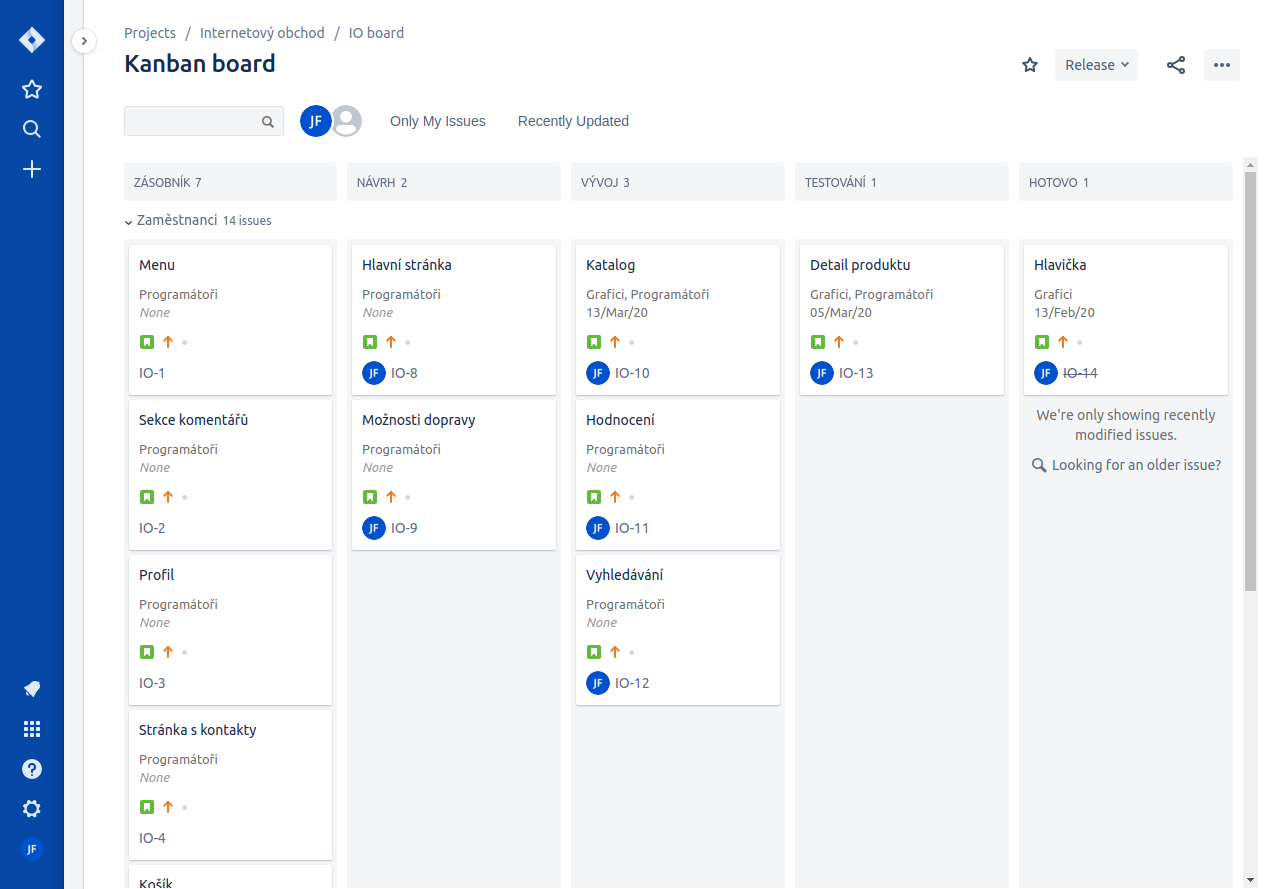
\includegraphics[width=\textwidth]{obrazky-figures/jira.png}
	\caption{Vzorová Kanban nástěnka ve webové aplikaci Jira Software zaměřená na vývoj internetového obchodu.}
\end{figure}

\subsection{Kanboard}
Kanboard\footnote{Kanboard: \url{https://kanboard.org}} je bezplatná webová aplikace s otevřeným zdrojovým kódem. Jejím tvůrcem je Frédéric Guillot, nicméně zdrojové kódy jsou volně k dispozici na portálu GitHub\footnote{Repozitář Kanboard na platformě GitHub: \url{https://github.com/kanboard/kanboard}}, kde se k vývoji připojilo dalších 270 lidí~\cite{bib:kanboard-github}. Aplikace je napsaná především v jazyce PHP a JavaScript. K provozování této aplikace je nutné použít vlastní webový server. Kanboard uživatelům nenabízí žádné přepychové uživatelské rozhraní, ale naopak se zaměřuje na jednoduchost a minimalismus~\cite{bib:kanboard}.

Mimo základní funkce metodiky Kanban tato aplikace umožňuje také vyhledávat úkoly za pomocí vlastního dotazovacího jazyka. Částečně také umožňuje práci s nástěnkou automatizovat pomocí konfigurovatelných akcí.

Vzhledem k otevřenému zdrojovému kódu lze aplikaci v případě potřeby upravit na míru vlastním potřebám. Součástí aplikace je však i rozhraní pro zásuvné moduly. Několik takových modulů lze nalézt i přímo na oficiální stránce\footnote{Zásuvné moduly pro Kanboard: \url{https://kanboard.org/plugins.html}}, avšak nepodléhají žádnému schvalovacímu procesu a není zaručena jejich kompatibilita.

\begin{figure}[H]
	\centering
	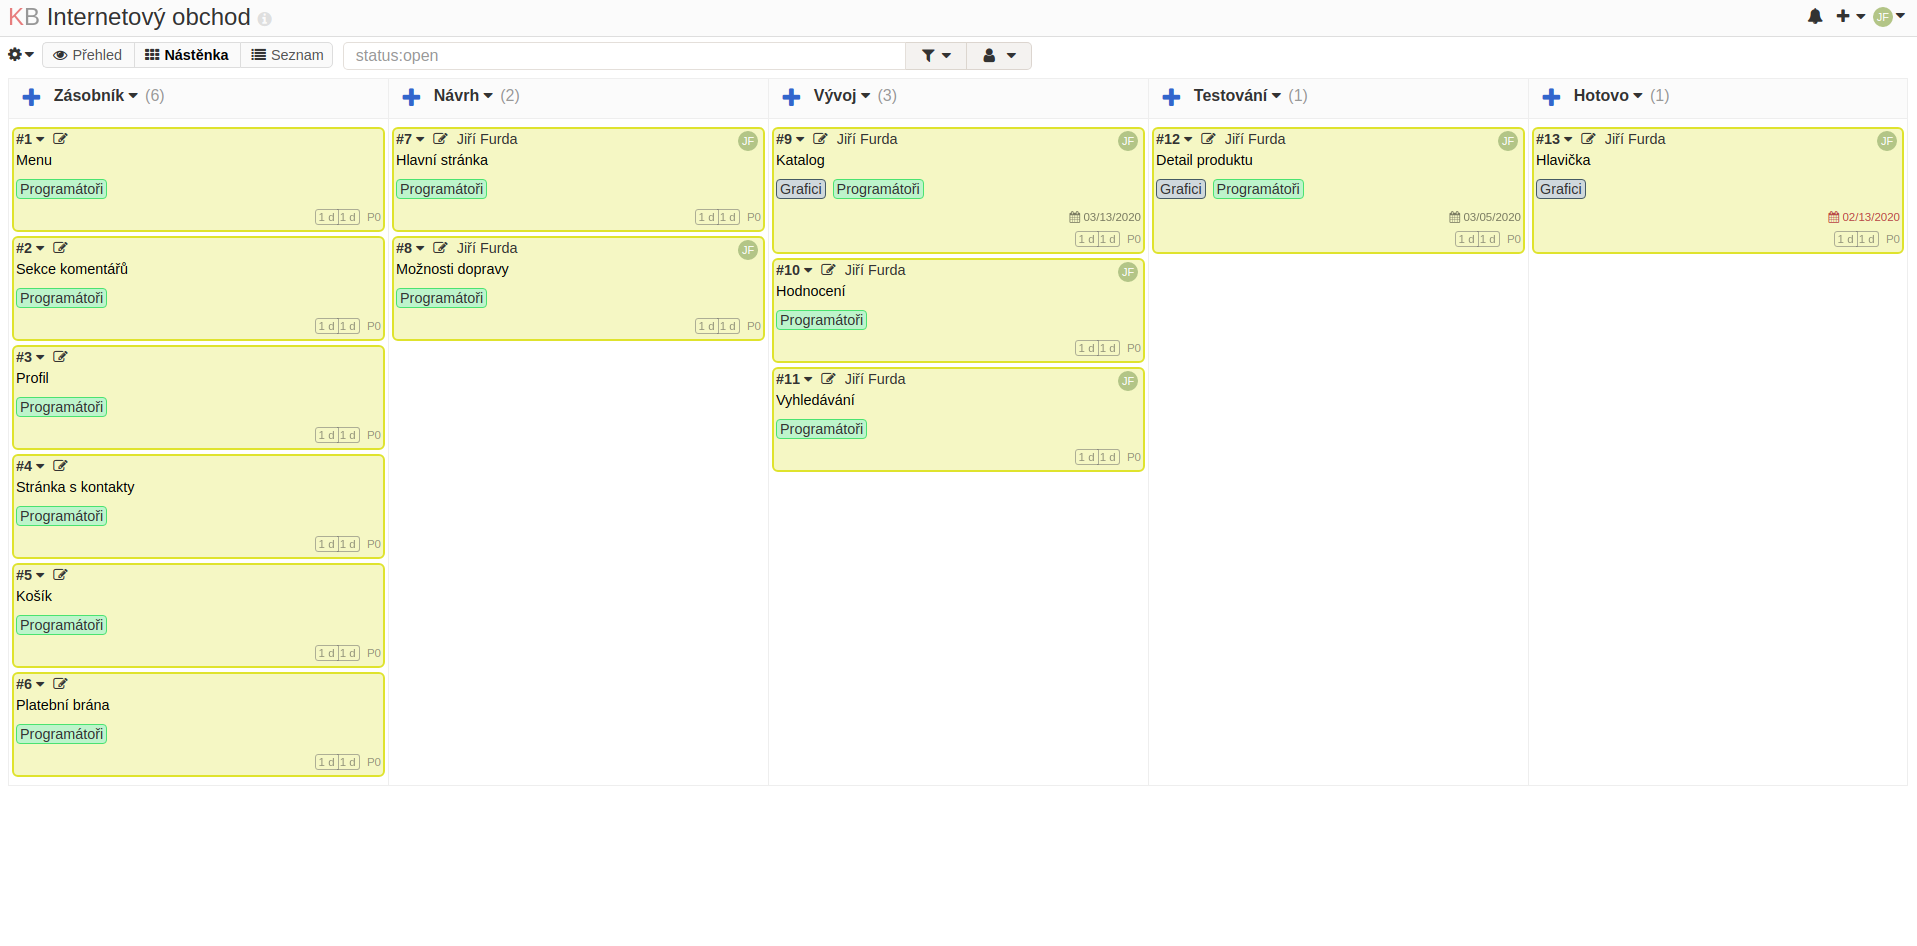
\includegraphics[width=\textwidth]{obrazky-figures/kanboard.png}
	\caption{Vzorová Kanban nástěnka ve webové aplikaci Kanboard zaměřená na vývoj internetového obchodu.}
\end{figure}

\subsection{Souhrn rozdílů}
Z důvodu ochrany firemního tajemství mohou být preferovány služby Jira a Kanboard, jelikož je možné je provozovat přímo na svém vlastním serveru. Konkrétně u aplikace Kaboard může tato vlastnost však představovat pro řadu uživatelů nevýhodu. Aplikaci totiž není možné jednoduše provozovat na vzdáleném úložišti. Uživatel musí mít k dispozici server, kde bude aplikace provozována a to se může stát barierou pro méně pokročilé uživatele počítače.

Kanboard však jako jediná z tří uvedených aplikací má otevřený zdrojový kód. Umožňuje tak větší úpravy aplikace než v případě dalších dvou, kde lze úpravy řešit pouze pomocí doplňků.


\blindtext


Slabší stránka aplikace Kanboard je na první pohled uživatelského rozhraní. Nejedná se však pouze o vzhled aplikace. Rozhraní obsahuje i mnoho prvků, které nejsou řešeny pomocí asynchronních požadavků, a to může být uživateli vnímáno jako nepohodlné či zastaralé.

% @todo https://www.atlassian.com/customers nekam vecpat 83% of Fortune 500 companies use Atlassian products

\section{Představení zadavatele}
\blindtext

\subsection{Současný produkt}
Jedním z mnoha produktů společnosti SEACOMP s.r.o. je systém SSB (SEACOMP SYSTEM BUILDER), určený pro snadnou tvorbu komplexních informačních systémů. Jedná se o počítačový program napsaný za použití technologie .NET.

V loňském roce se v rámci své diplomové práce Bc. Adam Teršl věnoval implementaci webového klienta pro tento systém. Výsledkem jeho snažení byla webová aplikace SSB4Web využívající především systém Angular. Aplikace je schopna komunikovat se serverem systému SSB a díky zásuvným modulů umožňuje prezentaci základních typů dat, které tvoří základ tohoto systému~\cite{bib:tersl}. Stolní verze klienta však obsahuje celou řadu dalších specializovaných zásuvných modulů, které pro webovou verzi klienta dosud nebyly implementovány. Jedním z těchto modulů je právě nástroj \emph{KANBAN board} pro optimalizaci spolupráce týmů, jehož implementace je cílem mé práce~\cite{bib:seacomp-portfolio}. 

\subsection{Požadavky na aplikaci}
Původní nástroj \emph{KANBAN board} však svou funkcionalitou pro pokročilejší řízení projektů již nestačí. Z tohoto důvodu se v rámci interního projektového řízení začal ve společnosti SeaComp používat nástroj Kanboard, který byl upraven a obohacen o některé specializované funkce. Tento nástroj však pracuje mimo ekosystém SSB. Přáním společnosti je mít k dispozici nástroj, který umožňuje pokročilejší práci s nástěnkou typu Kanban a tento nástroj mít plně integrován do produktu SSB4Web. Z tohoto důvodu bylo vypsané toto téma bakalářské práce.

Z důvodu ochrany obchodního tajemství však není možné zveřejnit zdrojové kódy programu SSB. Pro řešení této bakalářské práce je tudíž nejprve nutné vytvořit zjednodušenou verzi toho systému. Ta nese označení SSBLite a dle požadavku zadavatele je psána v jazyce C\#, konkrétně za použití ASP.Net Core. Tato část slouží jako server a komunikuje s klienty skrze aplikační rozhraní REST.

Podoba aplikačního rozhraní z důvodu budoucí integrace do systému SSB4Web musí odpovídat podobě používané právě v této zmíněné webové aplikaci. Samotná integrace však na přání společnosti není předmětem této práce, aplikaci je proto i přes budoucí integraci nutno vytvořit jako samostatnou webovou aplikaci obsahující například i autentizaci uživatelů a další komponenty.

Dále je požadováno, aby webová aplikace používala stejné technologie jako původní SSB4Web, tedy systém Angular s knihovnou pro správu stavu NgRx. Výjimkou je v tomto případě knihovna použitá pro uživatelské rozhraní, kdy původní diplomová práce využívala knihovnu PrimeNG\footnote{PrimeNG: \url{https://primefaces.org/primeng/}}. Po dokončení této práce však bylo společností požadováno knihovnu nahradit za balík komponent DevExtreme. Tento balík je tedy při implementaci práce rovněž využít.

Od samotné funkcionality aplikace je očekáváno \blindtext

\section{Technologie}
V této podkapitole jsou ve stručnosti přiblíženy technologie a techniky využité při tvorbě této práce. 

Úvod podkapitoly je věnován klientské části aplikace. Je zde popsán princip jednostránkových aplikací, programovací jazyk JavaScript, jeho typová nástavba TypeScript, systém Angular a jeho knihovny NgRx a DevExtreme.

Dále jsou zmíněny technologie zajišťující propojení klientské části aplikace s části serverovou. Toho je docíleno díky aplikačnímu rozhraní REST a metody JWT, která zajišťuje autentizaci uživatelů a autorizaci jejich požadavků.

V poslední části podkapitoly je zase popsána serverová část. Ta se skládá z technologie ASP.NET, která zpracovává požadavky zaslané z klientské části aplikace a překládá je na dotazy databáze, která využívá technologii PostgreSQL.


\subsection{Jednostránkové aplikace}

\emph{Tato kapitola čerpá z~\cite{bib:spa}}.

V raných dobách internetu se webové stránky skládaly ze statického obsahu. S popularizací elektronického obchodování se však objevila potřeba na stránkách zobrazovat i obsah dynamický. 
Toho lze docílit například díky technologii AJAX (Asynchronous JavaScript and XML). Jednostránkové aplikace se zpravidla skládají z komponent, které lze nezávisle nahradit nebo aktualizovat. Díky tomu není nutné při každé akci znovu načíst celou stránku, čímž je značně zredukován objem přenášených dat. Ve srovnání s vícestránkovými aplikacemi tak tento přístup umožňuje rychleji reagovat na požadavky uživatele.

\blindtext %todo vic se rozepsat

\subsection{JavaScript}
\blindtext

\subsubsection{TypeScript}
Samotný jazyk JavaScript však pro vývojáře může představovat překážku při implementaci rozsáhlých aplikací. %todo Proč
Řešením tohoto problému je například nástavba TypeScript, která tento jazyk obohacuje o prvky běžně používané v jiných programovacích jazycích. Jedná se ku příkladu o moduly, třídy, rozhraní a statické typování~\cite{bib:typescript}.
 
Jelikož internetové prohlížeče jazyk TypeScript neznají, je využíván překladač, který kód překládá do jazyka JavaScript.

\blindtext

\subsection{Angular}
Angular je webová platforma umožňující tvorbu jednostránkových aplikací s využitím jazyků TypeScript a HTML. Tato platforma si velmi zakládá na modularizaci kódu.
\blindtext[2] % https://angular.io/guide/architecture

% @todo https://www.angularjswiki.com/angular/history-of-angularjs/
Autorem platformy Angular je Miško Hevery, zaměstnanec společnosti Google. Platformu původně psal pro usnadnění vývoje několika interních projektů. V roce 2010 však byla platforma i její zdrojový kód otevřena široké veřejnosti. V následujících letech se oblast vývoje webových aplikací změnila a Angular již nedokázal držet krok. Platforma se stala velmi populární, s čímž původní návrh nepočítal. Bylo tedy nutné platformu Angular kompletně přepsat. Na podzim roku 2016 byla vydána nová verze této platformy s označením Angular 2. K dnešnímu dni se nové verze dostaly až k označení pod číslem 9, nicméně se stále jedna o rozšíření původního jádra verze 2. Na vývoji se stále podílí jak společnost Google, tak i komunita. Pro odlišení původní verze od nových přepsaných verzí se ta původní označuje jako AngularJS~\cite{bib:angular-history}.

\subsubsection{NgRx}
NgRx je systém pro správu stavu určený pro platformu Angular. Tento systém je založen na principu Redux.
\blindtext % @todo popsat o co jde 
% https://books.google.cz/books?hl=cs&lr=&id=OLZTDwAAQBAJ&oi=fnd&pg=PP1&dq=ngrx&ots=HoiBNWn4zq&sig=zrkpeOuKBmhqnd1ojsGeasbym7g&redir_esc=y#v=onepage&q=boiler&f=false

Tento systém však pro tvorbu aplikací pomocí platformy Angular potřeba nutně potřeba a v některých případech může i přitížit. I přes veškeré výhody, které využití tohoto systému přináší, je třeba počítat i s negativními následky. Systém má poměrně strmou učební křivku a je třeba znát princip Redux a umět používat knihovnu RxJS~\cite{bib:ngrx-docs}.
Dalším úskalím je velké množství přebytečného kódu. Přidání zdánlivě jednoduché funkce může trvat delší dobu, protože sebou nese nutnost přidat spoustu kódu napříč různými soubory. Proto je dobré nejprve důkladně zvážit, zda je vhodné pro daný projekt tento systém využít. Vývojáři systému NgRx proto na jedné z konferencí\footnote {ng-conf 2018 - Reducing the Boilerplate with NgRx: \url{https://www.youtube.com/watch?v=t3jx0EC-Y3c}} přišli se zásadou SHARI, které toto rozhodnutí usnadní. 

Zásada SHARI:
\begin{itemize}
  \item Sdílení (angl. shared) - Ke stavu přistupuje více komponent a služeb
  \item (angl. hydrated) - Stav přetrvává a je obnovován z externího zdroje
  \item (angl. available) - 
  \item (angl. retrieved) - 
  \item (angl. impacted) - 
\end{itemize}

\blindtext
\begin{figure}[H]
	\centering
	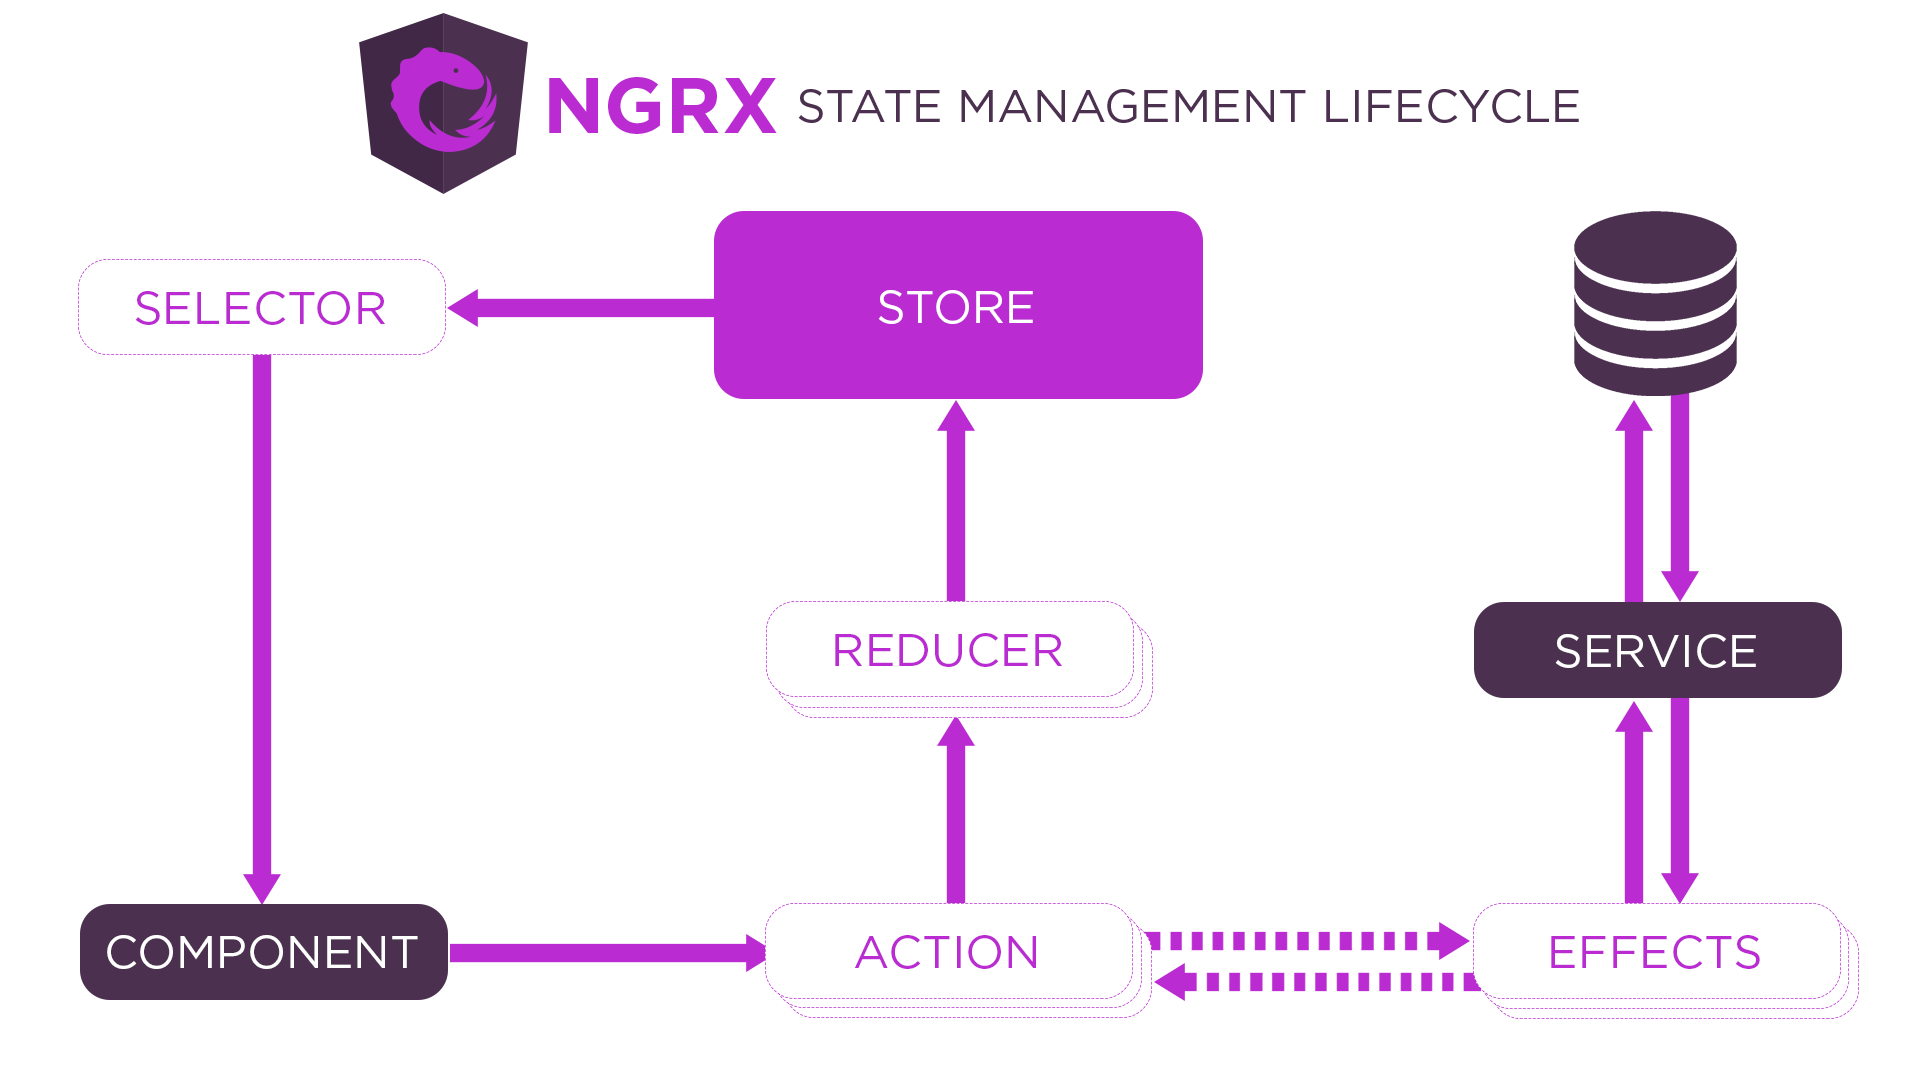
\includegraphics[width=\textwidth]{obrazky-figures/ngrx-lifecycle.png}
	\caption{Životní cyklus správy stavu s využitím knihovny NgRx. @todo popsat uzly \emph{Převzato z~\cite{bib:ngrx-lifecycle}}.}
\end{figure}
\blindtext

\subsubsection{DevExtreme}
DevExtreme je balík komponent určený pro tvorbu responzivních webových aplikací. Je k dispozici pro knihovny jQuery, Konockout, AngularJS, Angular, Vue, React, ASP.NET MVC 5 a ASP.NET Core.  
\blindtext

\subsection{REST}
\blindtext[2]

\subsection{JSON Web Token}
JSON Web Token (zkráceně JWT) je standard\footnote{RFC 7519: \url{https://tools.ietf.org/html/rfc7519}} zajišťující zabezpečenou výměnu informací mezi dvěma stranami. 
\blindtext

\subsection{ASP.NET Core}
ASP.NET Core je platforma společnosti Microsoft určena pro tvorbu webových aplikací. Jedná se o rozšíření populární platformy .NET určené především pro programovací jazyk C\#, taktéž vyvinutým společností Microsoft.

Přestože tato společnost stojí za dnes nejpopulárnějším operačním systémem Windows, je platformu ASP.NET Core možné provozovat i na jiných operačních systémech. Vydání první verze této platformy proběhlo v roce 2016~\cite{bib:asp-release}, dříve bylo možné platformu využít pouze na operačním systému Windows, tyto dřívější verze nesly název pouze ASP.NET bez označení Core~\cite{bib:asp-what-is}.

\blindtext

\subsection{PostgreSQL}
\blindtext

\chapter{Návrh aplikace}
\blindtext

\section{Schéma systému}
\blindtext
\begin{figure}[H]
	\centering
	
\includegraphics[width=\textwidth]{obrazky-figures/placeholder.pdf}
\end{figure}

\section{Diagram případů užití}
\blindtext
\begin{figure}[H]
	\centering
	
\includegraphics[width=\textwidth]{obrazky-figures/placeholder.pdf}
\end{figure}

\section{Entitně-vztahový diagram}
\blindtext
\begin{figure}[H]
	\centering
	
\includegraphics[width=\textwidth]{obrazky-figures/placeholder.pdf}
\end{figure}

\section{Grafický návrh}
\blindtext
\begin{figure}[H]
	\centering
	
\includegraphics[width=\textwidth]{obrazky-figures/placeholder.pdf}
\end{figure}


\section{Aplikační rozhraní}
\blindtext[2]

\chapter{Implementace aplikace}
Předmětem této kapitoly\blindtext

\section{Klientská část}

\section{Serverová část}

Z důvodu zachování firemního tajemství klientská část mé práce nekomunikuje přímo se systémem SSB, ale pouze se zjednodušenou verzí zvanou SSBLite, kterou jsem vytvořil v rámci řešení této bakalářské práce. Jedná se o webový server vytvořený s použitím systému ASP.Net. Server zpracovává požadavky aplikačního rozhraní REST na základě kterých sestrojuje a odesílá požadavky na databázi. Výsledky těchto požadavků jsou poté odeslány zpět klientovi ke zpracování a zobrazení uživateli.

Samotný webový server neobsahuje aplikační logiku, slouží pouze jako zprostředkovatel přístupu k databázi, ke které klient z důvodu bezpečnosti nesmí mít přímý přístup. Možné požadavky na databázi jsou předem určeny a uloženy v konfiguračních souborech. Díky tomu je možné v budoucnu upravit chování aplikace bez nutnosti přímého zásahu do zdrojového kódu serverové části aplikace. 

Konfigurační soubory využívají formát JSON a obsahují názvy jednotlivých požadavků a jejich znění. To však v mnoha případech přímo neobsahuje platný dotaz na databázi, ale obsažený dotaz je obohacen o klíčová slova, která umožňují přizpůsobení jeho znění pro aktuální potřebu klienta. Před samotným odesláním dotazu do databáze je nutné tyto klíčová slova zpracovat. Příkladem, využívajícím klíčové slovo \texttt{\{WHERE\}}, je následující dotaz:
\begin{verbatim}
{
    "name": "getCards",
    "content": "SELECT car.* FROM cards car JOIN columns col ON col.id = 
        car.column_id JOIN boards boa ON boa.id = col.board_id {WHERE}"
},
\end{verbatim}

\subsection{Databázová vrstva}

\chapter{Vyhodnocení}


\chapter{Závěr}